\subsection{Ice temperature profile}\label{sec:IceTemperatureProfile}
\chapterauthor{Kristian Sloth Lauszus and Lukas Christensen}

%* Indirect: salinity, melting speed
%* Drill sample
%* Passive screw in the tip
%	* Thermal isolated
%* Measure heat conductivity of the water
%	* Can be used to estimate the salinity of the water
%		* Melting speed
%
%* "back of the envelope" calculations

In order to estimate the descent time it is important to know the ice temperature profile i.e. the temperature change as a function of the depth and the energy required in order to melt the column of ice. The thermal conductivity of polycrystalline ice can be calculated according to the following equation\cite[(2.3)]{article:thermalConductivity}:
\begin{equation}
	k(T) = \frac{a_1}{T} + a_0
\end{equation}
Where the constants $a_1$ and $a_0$ are given by:
\begin{align}
	a_1 &= \unitfrac[4.88 \e7]{ergs}{cm \, s} \\ \nonumber
		&= \unitfrac[488]{W}{m} \\
	a_0 &= \unitfrac[4.68 \e4]{ergs}{cm \, K \, s} \\ \nonumber
		&= \unitfrac[0.468]{W}{m \, K}
\end{align}
The boundary conditions for the temperature is simply given by 273.15 K at the transition between the water and ice and 100 K at the surface of the moon\cite{article:thermalConductivity}. Thus the temperature difference can be calculated:
\begin{align}
	& T_m = \unit[273.15]{K} \\
	& T_s = \unit[100]{K} \\
	& T_\Delta = T_m - T_s = \unit[173.15]{K}
\end{align}
Figure \ref{fig:T_vs_k} shows two plots of the thermal conductivity as a function of the temperature. Figure \ref{fig:T_vs_k_full} shows the thermal conductivity from 0 K to 273.15 K, figure \ref{fig:T_vs_k_zoom} on the other hand shows only shows the thermal conductivity in the range of the boundary conditions.
\begin{figure}[htb]
	\centering
	\subfloat[From 0 K to 273.15 K]{
		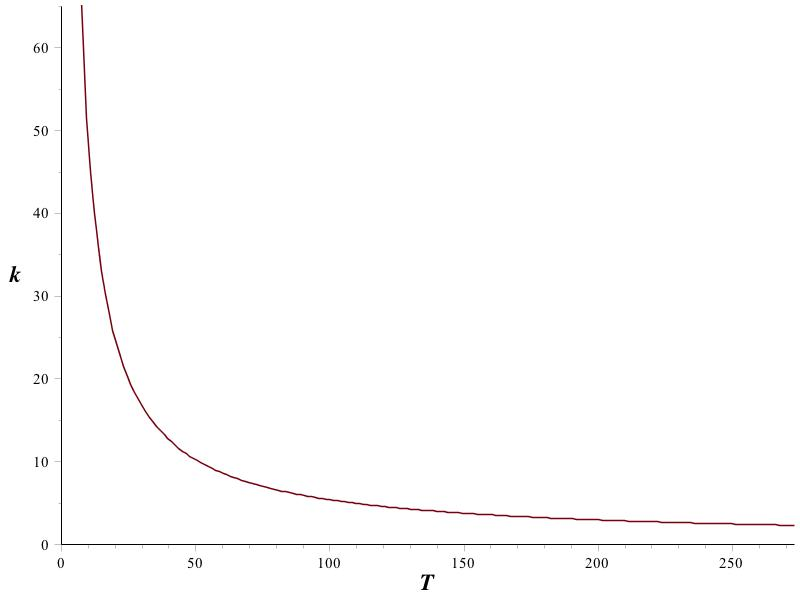
\includegraphics[width=.48\textwidth]{figures/temperature/T_vs_k}
		\label{fig:T_vs_k_full}
	}
	\subfloat[From $T_s$ to $T_m$]{
		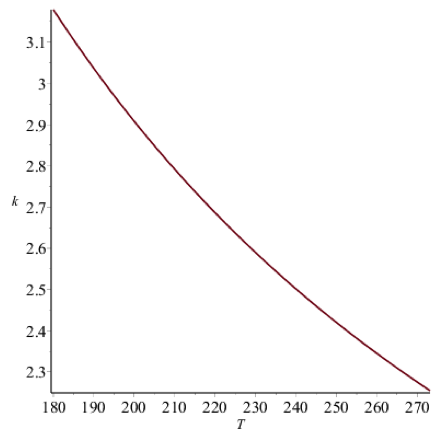
\includegraphics[width=.48\textwidth]{figures/temperature/T_vs_k_zoom}
		\label{fig:T_vs_k_zoom}
	}
	\caption{Thermal conductivity as a function of the temperature}
	\label{fig:T_vs_k}
\end{figure}
The conductive heat transfer can be calculated fairly easily using Fourier's Law\cite{website:conductiveHeatTransfer}:
\begin{align}
	q(T) &= \frac{k(T) A T_\Delta}{d}
\end{align}
The area $A$ is the area of the penetrator facing the ice and by assuming a cylinder with a radius of 10 cm the area is given by:
\begin{align}
	A &= \pi \, 0.1^2 \approx \unit[0.03]{m^2}
\end{align}
Figure \ref{fig:T_vs_q} shows a plot of the conductive heat transfer as a function of the temperature. The thickness of the ice $d$ is assumed to be 3 km according to chapter \ref{sec:structural_profile}.
\begin{figure}[htb]
	\centering
	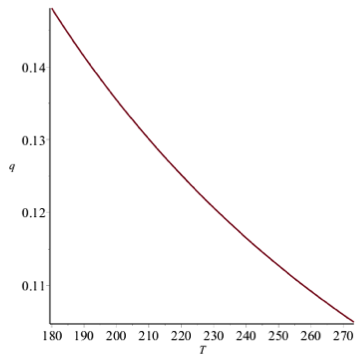
\includegraphics[width=.48\textwidth]{figures/temperature/T_vs_q}
	\caption{Conductive heat transfer as a function of the temperature}
	\label{fig:T_vs_q}
\end{figure}
Notice how both the conductive heat transfer $q$ and the thermal conductivity $k$ are approximately constant doing the interval $T_s$ to $T_m$, thus they can both be approximated by the average over the interval:
\begin{align}
	\bar{k} &= \unitfrac[3.80]{W}{m \, K} \\
	\bar{q} &= \unit[0.0066]{W}
\end{align}
Now the temperature as a function of the depth $d$ can be calculated assuming that the heat transfer and thermal conductivity are constant throughout the ice:
\begin{align}\label{eq:T_d}
	T(d) &= T_s + d \frac{\bar{q}}{\bar{k} A} = 100 K + \unitfrac[0.058 d]{K}{m}
\end{align}
Figure \ref{fig:d_vs_T} shows a plot of the temperature as a function of the depth into the ice.
\begin{figure}[htb]
	\centering
	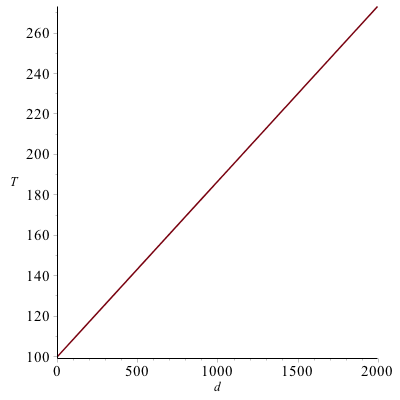
\includegraphics[width=.48\textwidth]{figures/temperature/d_vs_T}
	\caption{Temperature as a function of the depth}
	\label{fig:d_vs_T}
\end{figure}
\\
Figure \ref{fig:T_vs_rho} shows the density of ice as a function of the temperature using the values found in Table \ref{tab:ice_density}. This is be approximated by a linear second order function:
\begin{equation}\label{eq:rho_approx}
	\rho(T) = 931.21 - 0.68 \e{-3} T - 0.19 \e{-3} T^2
\end{equation}
Figure \ref{fig:T_vs_rho_approx} shows a plot of the approximated density of ice as a function of the temperature.

\begin{figure}[htb]
	\centering
	\subfloat[Density of ice according to Table \ref{tab:ice_density}]{
		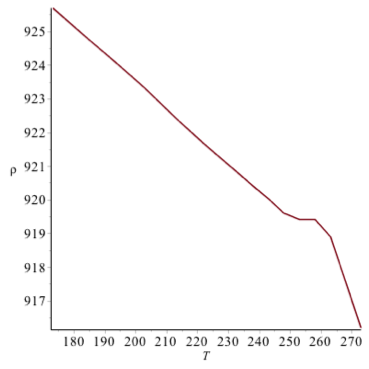
\includegraphics[width=.48\textwidth]{figures/temperature/T_vs_rho}
		\label{fig:T_vs_rho}
	}
	\subfloat[Approximated ice density using \eqref{eq:rho_approx}]{
		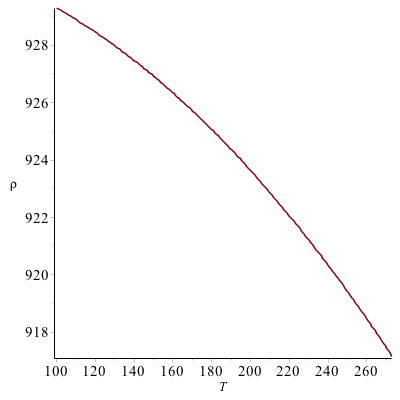
\includegraphics[width=.48\textwidth]{figures/temperature/T_vs_rho_approx}
		\label{fig:T_vs_rho_approx}
	}
	\caption{Density of ice as a function of the temperature}
\end{figure}

\noindent
Now the density as a function of the distance can be calculated by inserting \eqref{eq:T_d} into \eqref{eq:rho_approx}:
\begin{equation}\label{eq:rho_approx_d}
	\rho(d) = 929.29 - 0.22 \e{-2} d - 6.19 \e{-7} d^2
\end{equation}
%A plot of \eqref{eq:rho_approx_d} and \eqref{eq:T_diff} can be seen in Figure \ref{fig:d_vs_rho} and Figure \ref{fig:d_vs_T_delta} respectively.
%\begin{figure}[htb]
%	\centering
%	\captionsetup[subfigure]{width=0.45\textwidth}
%	\subfloat[Ice density as a function of the depth using \eqref{eq:rho_approx_d}]{
%		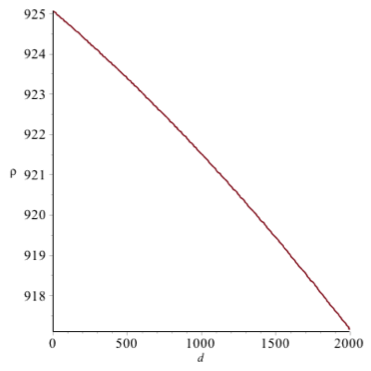
\includegraphics[width=.48\textwidth]{figures/temperature/d_vs_rho}
%		\label{fig:d_vs_rho}
%	}
%	\subfloat[Temperature difference as a function of the depth]{
%		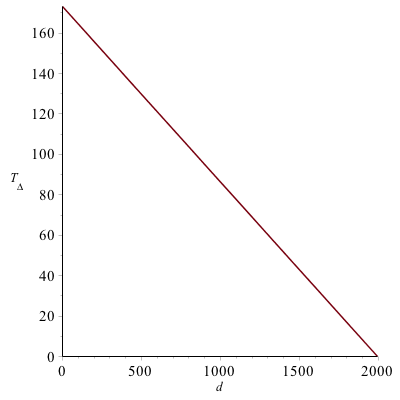
\includegraphics[width=.48\textwidth]{figures/temperature/d_vs_T_delta}
%		\label{fig:d_vs_T_delta}
%	}
%	\caption{}
%\end{figure}

\begin{wraptable}{R}{0pt}
	\centering
	\begin{tabular}{|c|c|}
		\hline
		T (K) & $\rho$ ($\unitfrac{kg}{m^3}$) \\ \hline
		273.15 & 916.2 \\ \hline
		268.15 & 917.5 \\ \hline
		263.15 & 918.9 \\ \hline
		258.15 & 919.4 \\ \hline
		253.15 & 919.4 \\ \hline
		248.15 & 919.6 \\ \hline
		243.15 & 920.0 \\ \hline
		238.15 & 920.4 \\ \hline
		233.15 & 920.8 \\ \hline
		223.15 & 921.6 \\ \hline
		213.15 & 922.4 \\ \hline
		203.15 & 923.3 \\ \hline
		193.15 & 924.1 \\ \hline
		183.15 & 924.9 \\ \hline
		173.15 & 925.7 \\ \hline
	\end{tabular}
	\caption{Density of ice for different temperatures\cite{website:iceDensity}}
	\label{tab:ice_density}
\end{wraptable}
\noindent
Figure \ref{fig:T_vs_Cice} shows the specific heat capacity of ice plotted using the data found in Table \ref{tab:ice_heat_capacity}. Again this is approximated using a linear second order function:
\begin{equation}\label{eq:Cice_approx}
	C_{ice}(T) = -372.95 + 12.34 T - 0.013 T^2
\end{equation}
The specific heat capacity of ice as a function of the distance can be calculated by inserting \eqref{eq:T_d} into \eqref{eq:Cice_approx}:
\begin{equation}\label{eq:Cice_approx_d}
	C_{ice}(d) = 734.76 + 0.57 d - 0.42 \e{-4} d^2
\end{equation}
A plot of the approximated specific heat capacity can be seen in Figure \ref{fig:T_vs_Cice_approx}.

\begin{wraptable}{R}{0pt}
	\centering
	\begin{tabular}{|c|c|}
		\hline
		T (K) & $C_{ice}$ ($\unitfrac{J}{K \, kg}$) \\ \hline
		273.15 & 2050 \\ \hline
		268.15 & 2027 \\ \hline
		263.15 & 2000 \\ \hline
		258.15 & 1972 \\ \hline
		253.15 & 1943 \\ \hline
		248.15 & 1913 \\ \hline
		243.15 & 1882 \\ \hline
		238.15 & 1851 \\ \hline
		233.15 & 1818 \\ \hline
		223.15 & 1751 \\ \hline
		213.15 & 1681 \\ \hline
		203.15 & 1609 \\ \hline
		193.15 & 1536 \\ \hline
		183.15 & 1463 \\ \hline
		173.15 & 1389 \\ \hline
	\end{tabular}
	\caption{Specific heat capacity of ice for different temperatures\cite{website:iceDensity}}
	\label{tab:ice_heat_capacity}
\end{wraptable}

\begin{figure}[!b]
	\centering
	\subfloat[Specific heat capacity of ice according to Table \ref{tab:ice_heat_capacity}]{
		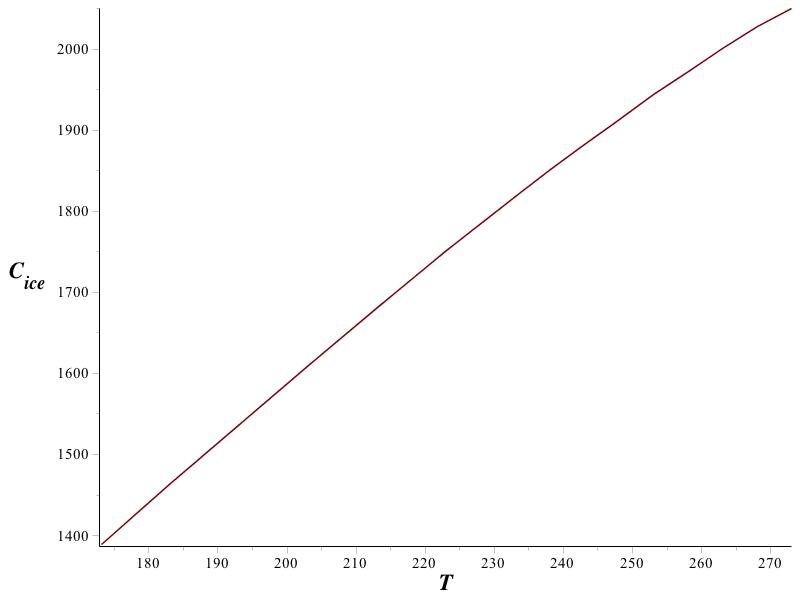
\includegraphics[width=.48\textwidth]{figures/temperature/T_vs_Cice}
		\label{fig:T_vs_Cice}
	}
	\subfloat[Approximated specific heat capacity of ice using \eqref{eq:Cice_approx}]{
		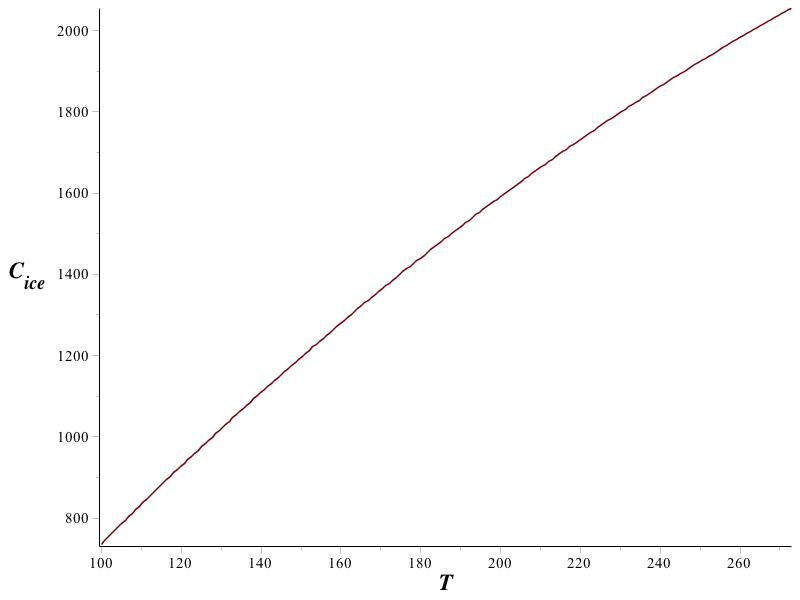
\includegraphics[width=.48\textwidth]{figures/temperature/T_vs_Cice_approx}
		\label{fig:T_vs_Cice_approx}
	}
	\caption{Specific heat capacity of ice as a function of the temperature}
\end{figure}

%\begin{figure}[htb]
%	\centering
%	\includegraphics[width=.48\textwidth]{figures/temperature/d_vs_C_ice}
%	\caption{Specific heat capacity of the depth}
%	\label{fig:d_vs_C_ice}
%\end{figure}

\noindent
The amount the temperature needs to be raised as a function of the distance is given by:
\begin{equation}\label{eq:T_diff}
	T_\Delta(d) = T_m - T(d) = 173.15 K - \unitfrac[0.058 d]{K}{m}
\end{equation}
The energy required to heat up the 3 km cylinder of ice to 0 \textdegree C can now be calculated:
\begin{align}
	E_0 &= A \, \int_0^{3\e{3}} \! C_{ice}(d) \, \rho(d) \, T_\Delta(d) \ \mathrm{d}d \\ \nonumber
	    &= \unit[8.93 \e{9}]{J}
\end{align}
The total mass of a 3 km cylinder of ice with an area of $A$ is given by:
\begin{equation}\label{eq:ice_total_mass}
	m_{total} = A \, \int_0^{3\e{3}} \! \rho(d) \ \mathrm{d}d = \unit[83174]{kg}
\end{equation}
Latent heat of melting of ice is given by\cite{website:waterLatentHeat}:
\begin{equation}
	L_m = \unitfrac[333.55 \e{3}]{J}{kg}
\end{equation}
The energy required for the phase change can now be calculated:
\begin{equation}
	E_{phase} = L_m m_{total} = \unit[2.77 \e{10}]{J}
\end{equation}
The total amount of energy is then given by:
\begin{equation}\label{eq:E_total}
	E_{total} = E_0 + E_{phase} = \unit[3.67 \e{10}]{J}
\end{equation}
It is noticeable that the energy required for the phase change takes up about 75 \% of the total energy, thus the approximations regarding the thermal conductivity, conductive heat transfer, and heat capacity should not have a huge impact on the result.

However the model of the ice density has a impact on the energy calculations of the phase change, as seen by \eqref{eq:ice_total_mass}. Thus a better model of the ice density would be beneficial. Further studies of the ice composition will be needed in this case, as the ice is assumed to be an isotropic and homogeneous material in the previous calculations. Furthermore the temperature at which the phase change occurs depends on the pressure as well.
% This will be discussed more in detail in chapter \ref{sec:temp_simulation}.
% Heat capacity and density is approximated below -100 C.

It is also noticeable that the energy required to melt the ice will be higher in practice than the total energy calculated in \eqref{eq:E_total}, as their will never be a 100 \% thermal energy transportation efficiency between the melting-device and the ice.

\subsubsection{Pressure Profile}

* What is the outside pressure?

\subsubsection{Simulation Results}\label{sec:temp_simulation}

\subsubsection{Simulation Validation}

* Should show that the "back of the envelope" calculations are right

\begin{figure}[htb]
	\centering
	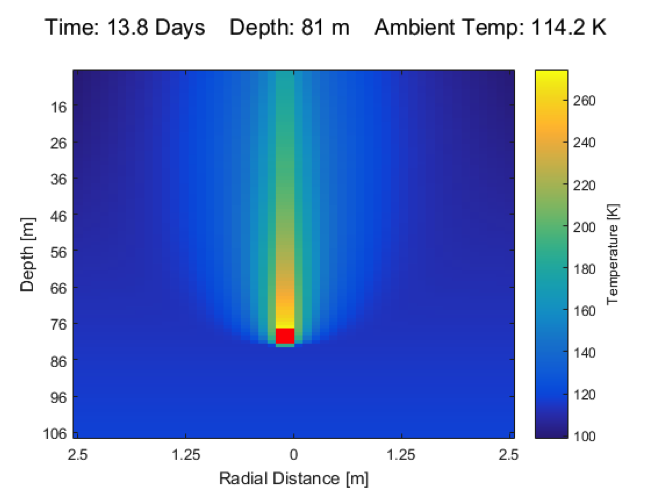
\includegraphics[width=\textwidth]{figures/temperature/temperature_simulation}
	\caption{TODO: Caption}
	\label{fig:temperature_simulation}
\end{figure}

\subsection{Water convection}

* Flow from tip to tail
* Passive water intake
	* Guided water intake
	* Flute shapes guides water as well
* Simulation
	* 3D model
	* CFD analysis

\begin{figure}[htb]
	\centering
	\subfloat[TODO: Caption]{
		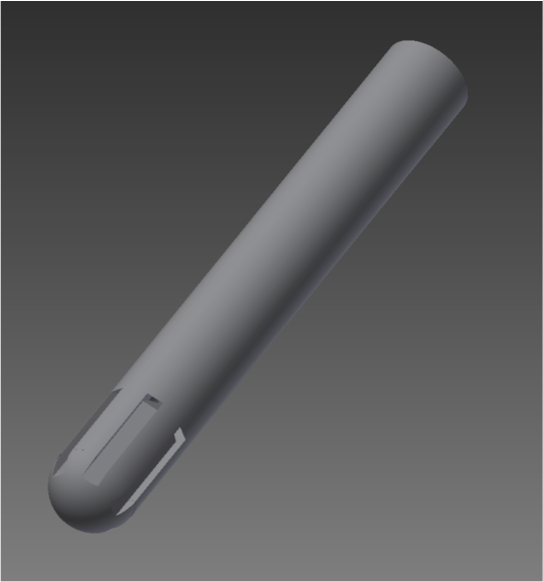
\includegraphics[width=.48\textwidth]{figures/convection/3d_model}
	}\\
	\subfloat[TODO: Caption]{
		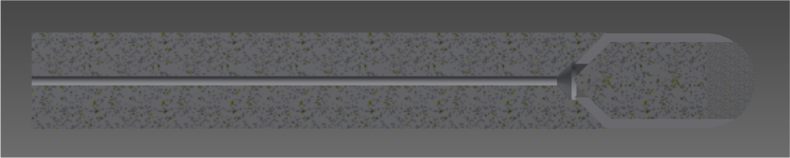
\includegraphics[width=.48\textwidth]{figures/convection/3d_model_inside}
	}
	\caption{TODO: Caption}
	\label{fig:3d_model}
\end{figure}

\begin{figure}[htb]
	\centering
	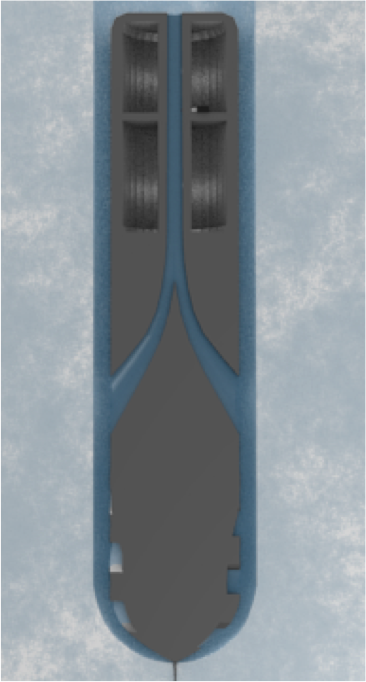
\includegraphics[width=.5\textwidth]{figures/convection/water_transportation}
	\caption{TODO: Caption}
	\label{fig:water_transportation}
\end{figure}

\subsubsection{CFD analysis}

* It is not enough!
	* Low Gravity!
	* 0.4 cm/s => 200 s/L
	* We will have to use a pump system

\begin{figure}[htb]
	\centering
	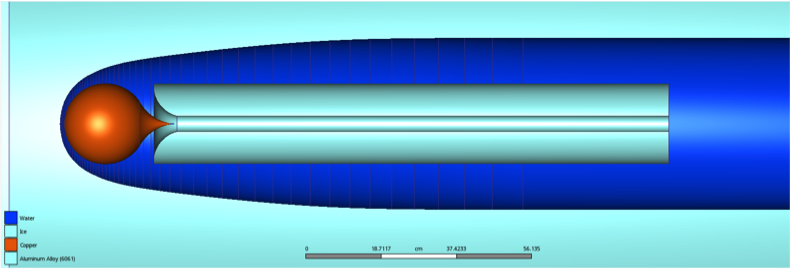
\includegraphics[width=\textwidth]{figures/convection/simplified_3d_model}
	\caption{TODO: Caption}
	\label{fig:simplified_3d_model}
\end{figure}

\begin{figure}[htb]
	\centering
	\subfloat[TODO: Caption]{
		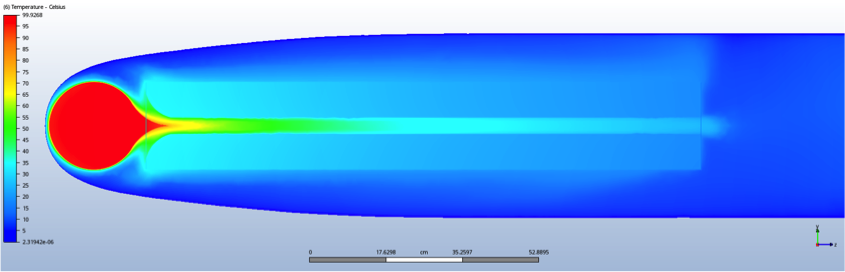
\includegraphics[width=.48\textwidth]{figures/convection/cfd_temperature}
	}
	\subfloat[TODO: Caption]{
		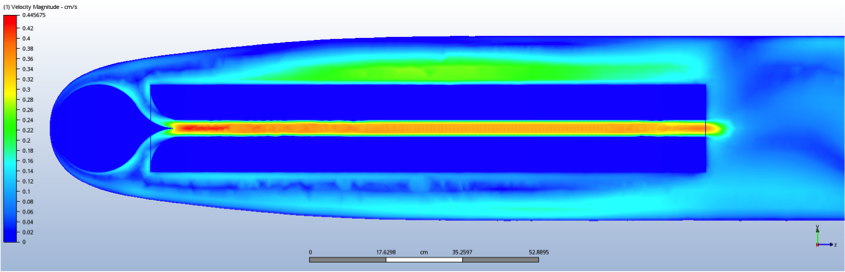
\includegraphics[width=.48\textwidth]{figures/convection/cfd_velocity}
	}
	\caption{TODO: Caption}
	\label{fig:cfd}
\end{figure}
